\begin{figure}[H]
  \centering
  \pgfplotsset{
  	    scaled y ticks=false,
    scale only axis,
    legend style={at={(0,0.8)}, anchor=west, font=\tiny},
    xmin=15,
  }
  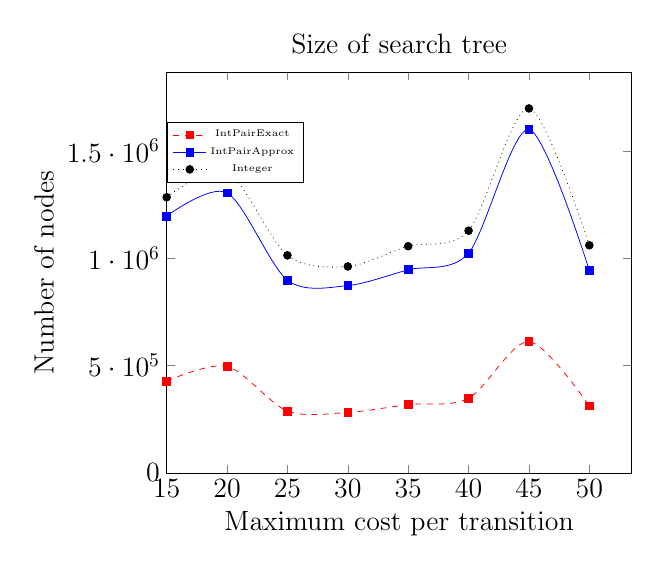
\begin{tikzpicture} [scale=0.7, font=\Large]
    \begin{axis}[
        title=Size of search tree,
        ylabel=Number of nodes,
        xtick=data,
        ymin=0, 
        xlabel=Maximum cost per transition ]
      \addplot[smooth,mark=square*, mark options={solid},red, dashed]
      coordinates{ (15,427514) (20,496441) (25,288296) (30,281590) (35,318147) (40,347192) (45,612036) (50,311950)
      }; %\label{ie_plot}
      \addlegendentry{IntPairExact}
      \addplot[smooth,mark=square*, mark options={solid},blue]
      coordinates{ (15,1195984) (20,1304175) (25,897266) (30,872190) (35,945941) (40,1023664) (45,1598498) (50,942876)
      }; %\label{ia_plot}
      \addlegendentry{IntPairApprox}
      \addplot[smooth,mark=*,mark options={solid},black, dotted]
      coordinates{ (15,1283617) (20,1403174) (25,1012948) (30,961248) (35,1055632) (40,1127914) (45,1696932) (50,1059848)
      }; %\label{int_plot}
      \addlegendentry{Integer}
    \end{axis}
  \end{tikzpicture}
  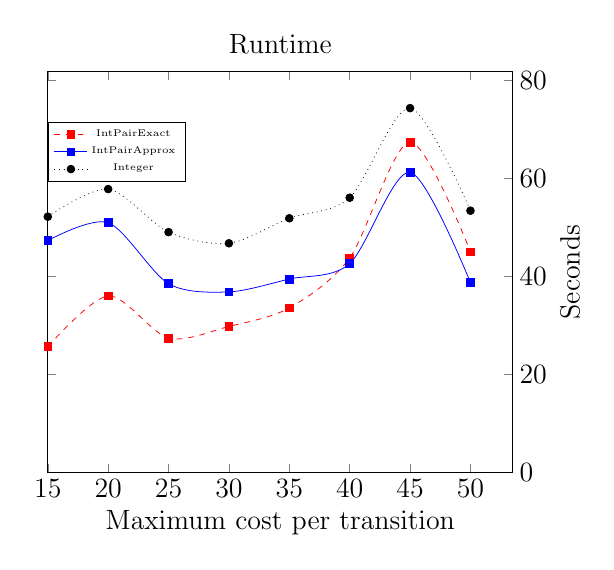
\begin{tikzpicture} [scale=0.7, font=\Large]
    \begin{axis}[
        yticklabel pos=right,
        xtick=data,
        title=Runtime,
        ylabel=Seconds,
        xlabel=Maximum cost per transition,
        ymin=0, ]
      \addplot[smooth,mark=square*,mark options={solid},red, dashed]
      coordinates{ (15, 25.684) (20, 36.053) (25, 27.456) (30, 29.816) (35, 33.596) (40, 43.801) (45, 67.417) (50, 45.049)
      };% \label{IntPairExact Run}
      \addplot[smooth,mark=square*,mark options={solid},blue]
      coordinates{ (15, 47.323) (20, 50.981) (25, 38.542) (30, 36.873) (35, 39.495) (40, 42.646) (45, 61.284) (50, 38.757)
      }; %\label{IntPairApprox Run}
      \addplot[smooth,mark=*,mark options={solid},black, dotted]
      coordinates{ (15, 52.210) (20, 57.838) (25, 49.062) (30, 46.785) (35, 51.887) (40, 56.075) (45, 74.353) (50, 53.431)
      }; %\label{IntegerRun}
      \addlegendentry{IntPairExact}
      \addlegendentry{IntPairApprox}
      \addlegendentry{Integer}
    \end{axis}
  \end{tikzpicture}

%  \begin{tikzpicture}[scale=1.4]
%    \draw[very thick] (-4,0) -- (4,0);
%    \draw[draw=white] (-5,-0.2) -- (5,-0.2);
%  \end{tikzpicture}


%  \begin{tikzpicture} [scale=0.8]
%    \begin{semilogyaxis}[
%        title=No nodes logarithmic scale,
%        ylabel=nodes,
%        xtick=data,
%        ymin=0, 
%        xlabel=cost ]
%     \addplot[smooth,mark=square*, mark options={solid},red, dashed]
%      coordinates{ (15,427514) (20,496441) (25,288296) (30,281590) (35,318147) (40,347192) (45,612036) (50,311950)
%      }; %\label{ie_plot}
%      \addlegendentry{IntPairExact}
%      \addplot[smooth,mark=square*, mark options={solid},blue]
%      coordinates{ (15,1195984) (20,1304175) (25,897266) (30,872190) (35,945941) (40,1023664) (45,1598498) (50,942876)
%      }; %\label{ia_plot}
%      \addlegendentry{IntPairApprox}
%      \addplot[smooth,mark=*,mark options={solid},black, dotted]
%      coordinates{ (15,1283617) (20,1403174) (25,1012948) (30,961248) (35,1055632) (40,1127914) (45,1696932) (50,1059848)
%      }; %\label{int_plot}
%      \addlegendentry{Integer}

%    \end{semilogyaxis}
%  \end{tikzpicture}
%  \begin{tikzpicture} [scale=0.8]
%    \begin{semilogyaxis}[
%        title=Runtime logaritmhic scale,
%        yticklabel pos=right,
%        xtick=data,
%        ylabel=runtime (ms),
%        xlabel=cost,
%        ymin=0,  ]
%      \addplot[smooth,mark=square*,mark options={solid},red, dashed]
%      coordinates{ (15, 25684) (20, 36053) (25, 27456) (30, 29816) (35, 33596) (40, 43801) (45, 67417) (50, 45049)
%      }; %\label{IntPairExact Run}
%      \addplot[smooth,mark=square*,mark options={solid},blue]
%      coordinates{ (15, 47323) (20, 50981) (25, 38542) (30, 36873) (35, 39495) (40, 42646) (45, 61284) (50, 38757)
%     }; %\label{IntPairApprox Run}
%      \addplot[smooth,mark=*,mark options={solid},black, dotted]
%      coordinates{ (15, 52210) (20, 57838) (25, 49062) (30, 46785) (35, 51887) (40, 56075) (45, 74353) (50, 53431)
%      }; %\label{IntegerRun}
%      \addlegendentry{IntPairExact}
%      \addlegendentry{IntPairApprox}
%      \addlegendentry{Integer}
%    \end{semilogyaxis}
%  \end{tikzpicture}
  \caption{Varying the maximum cost per transition. The other parameters are fixed. Size of alphabet=7, size of alphabet=7, and number of steps=7. The lack of an obvious dependence pattern between the x and y axis is because the maximum total cost also varies with the cost per transition.}\label{fig:cost}
\end{figure}
